%%%%%%%%%%%%%%%%%%%%%%%%%%%%%%%%%%%%%%%%%
% Short Sectioned Assignment
% LaTeX Template
% Version 1.0 (5/5/12)
%
% This template has been downloaded from:
% http://www.LaTeXTemplates.com
%
% Original author:
% Frits Wenneker (http://www.howtotex.com)
%
% License:
% CC BY-NC-SA 3.0 (http://creativecommons.org/licenses/by-nc-sa/3.0/)
%
%%%%%%%%%%%%%%%%%%%%%%%%%%%%%%%%%%%%%%%%%

%----------------------------------------------------------------------------------------
%	PACKAGES AND OTHER DOCUMENT CONFIGURATIONS
%----------------------------------------------------------------------------------------

\documentclass[paper=a4, fontsize=11pt]{scrartcl} % A4 paper and 11pt font size
\usepackage[utf8]{inputenc}
\usepackage[MeX]{polski}
\usepackage[T1]{fontenc} % Use 8-bit encoding that has 256 glyphs
\usepackage{fourier} % Use the Adobe Utopia font for the document - comment this line to return to the LaTeX default
 % English language/hyphenation
\usepackage{amsmath,amsfonts,amsthm} % Math packages
\usepackage{graphicx} %images
\usepackage{placeins}%for direct positioning
\usepackage{lipsum} % Used for inserting dummy 'Lorem ipsum' text into the template

\usepackage{sectsty} % Allows customizing section commands
\allsectionsfont{\centering \normalfont\scshape} % Make all sections centered, the default font and small caps

\usepackage{fancyhdr} % Custom headers and footers
\pagestyle{fancyplain} % Makes all pages in the document conform to the custom headers and footers
\fancyhead{} % No page header - if you want one, create it in the same way as the footers below
\fancyfoot[L]{} % Empty left footer
\fancyfoot[C]{} % Empty center footer
\fancyfoot[R]{\thepage} % Page numbering for right footer
\renewcommand{\headrulewidth}{0pt} % Remove header underlines
\renewcommand{\footrulewidth}{0pt} % Remove footer underlines
\setlength{\headheight}{13.6pt} % Customize the height of the header

\numberwithin{equation}{section} % Number equations within sections (i.e. 1.1, 1.2, 2.1, 2.2 instead of 1, 2, 3, 4)
\numberwithin{figure}{section} % Number figures within sections (i.e. 1.1, 1.2, 2.1, 2.2 instead of 1, 2, 3, 4)
\numberwithin{table}{section} % Number tables within sections (i.e. 1.1, 1.2, 2.1, 2.2 instead of 1, 2, 3, 4)

\setlength\parindent{0pt} % Removes all indentation from paragraphs - comment this line for an assignment with lots of text

%----------------------------------------------------------------------------------------
%	TITLE SECTION
%----------------------------------------------------------------------------------------

\newcommand{\horrule}[1]{\rule{\linewidth}{#1}} % Create horizontal rule command with 1 argument of height

\title{	
\normalfont \normalsize 
\textsc{Uniwersytet Wrocławski} \\ [25pt] % Your university, school and/or department name(s)
\horrule{0.5pt} \\[0.4cm] % Thin top horizontal rule
\huge Interpolacja Lagrange'a i Newtona \\
\large Pracownia 2.7 \\ % The assignment title
\horrule{2pt} \\[0.5cm] % Thick bottom horizontal rule
}

\author{Artur Derechowski} % Your name

\date{\normalsize\today} % Today's date or a custom date

\begin{document}

\maketitle % Print the title

%----------------------------------------------------------------------------------------
%	PROBLEM 1
%----------------------------------------------------------------------------------------

\section{Treść}
Zrealizować algorytmy obliczania wartości wielomianu podanego za pomocą wzoru interpolacyjnego
Lagrange’a oraz zamiany postaci Lagrange’a na postać Newtona. Porównać dokładności wyników uzyskanych
za pomocą obu wzorów m.in. dla funkcji ${f_1(x) = (1+25x^2)^{-1}}$
i ${f_2(x) = arctg(x)}$.

\subsection{Postać Lagrange'a}
Wielomian interpolujący ${n+1}$ punktów ${(x_0, y_0), (x_1, y_1), ... , (x_n, y_n)}$ można zapisać
w postaci interpolacyjnej Lagrange'a, danej wzorem:
\begin{align} 
 p(x)= \sum_{i=0}^{n} f_i L_i(x), &&	\label{lag}
 L_i(x) = \prod_{\substack{j=0 \\ j \neq i}}^n \frac{x-x_j}{x_i-x_j}
\end{align}

Można sprawdzić, że ten wielomian przyjmuje wartości $y_i$ w punktach $x_i$ oraz, że jest
stopnia $\leqslant n$
Jest to jedyny wielomian stopnia ${\leqslant n}$ interpolujący zadane punkty. \medbreak
 
\subsection{Postać Newtona}
Ten sam wielomian może zostać zapisany w postaci Newtona jako:
\begin{align} 
 p(x)= \sum_{i=0}^{n} a_i \prod_{j=0}^{i-1} (x-x_j), && \label{new}
 a_k = \sum_{i=0}^k \frac{f(x_i)} {\prod_{\substack{j=0, j \neq i}}^k (x_i - x_j)}
\end{align}
gdzie współczynniki ${a_i}$ są ilorazami różnicowymi, które można również definiować rekurencyjnie jako:

\begin{align}
a_i = f[x_0,..., x_i] &&
f[x_0,..., x_i] = \frac{f[x_0,..., x_{i-1}] - f[x_1,..., x_i]}{x_0 - x_i}
\end{align}

\section{Zamiana postaci Lagrange'a na postać Newtona}
Postać Lagrange'a podana we wzorze \ref{lag} może być również zapisana jako:
\begin{align} 
 p(x)= \sum_{i=0}^{n} \sigma_i \prod_{\substack{j=0 \\ j \neq i}}^n (x-x_j), &&	\label{lsig}
 \sigma_i = \frac{f(x_i)}{\prod_{\substack{j=0 \\ j \neq i}}^n (x_i-x_j)}
\end{align}

Mając zapisane $\sigma_i$ w tej postaci można poprzez proste przekształcenie otrzymać
również współczynniki w postaci Newtona.
\begin{align} 
 a_k = \sum_{i=0}^k \frac{f(x_i)} {\prod_{\substack{j=0, j \neq i}}^k (x_i - x_j)} \label{a}
 = \sum_{i=0}^k \sigma_i \prod_{j=k+1}^n (x_i-x_j)
\end{align}

Wtedy, z równań \ref{a} oraz \ref{new} postać Newtona wielomianu interpolacyjnego
dana jest wzorem:
\begin{align} 
 p(x)= \sum_{i=0}^{n} a_k \prod_{j=0}^{i-1} (x-x_j) \label{nsig}
 = \sum_{i=0}^k \frac{f(x_i)} {\prod_{\substack{j=0, j \neq i}}^k (x_i - x_j)} \prod_{j=0}^{i-1} (x-x_j)
\end{align}

W dalszej części pracy będą rozważane wzory na postać Newtona podane w równaniu
\ref{nsig} oraz na postać Lagrange'a w równaniu \ref{lsig}.

\section{Badane funkcje}

Wiadomo, że n-ty błąd interpolacji dany jest wzorem:
\begin{align} 
 f(x) - p(x) = \frac{f^{(n+1)}(\xi)}{(n+1)!} \prod_{i=0}^n (x-x_i)
\end{align}
zależy on więc od pochodnej n-tego stopnia funkcji $f$. 
Dobierzemy więc odpowiednie funkcje, dla których ta pochodna może być dowolnie duża
(przy rosnącym n), aby uwidocznić różnicę pomiędzy funkcją a wielomianem ją interpolującym.

\subsection{Runge}
Funkcja Rungego dana jest wzorem:
\begin{align}
 rg(x) = \frac{1}{1+25x^2} 
\end{align}
Można pokazać, że jej kolejne pochodne są rozbieżne, na przykład 10-ta pochodna
w pobliżu zera osiąga wartość ponad $2*10^13$.

\subsection{arctan(x)}
Kolejne pochodne funkcji $arctan$ również gwałtownie rozbiegają w pobliżu zera,
dla przykładu 10-ta pochodna osiąga wartość ponad $2*10^5$. Można zauważyć, 
że zasada działania jest podobna do tej dla funkcji Rungego, ponieważ 
\begin{align}
 (arctan(x))' = \frac{1}{1+x^2}
\end{align}
czyli również ma $1+x^2$ w mianowniku i stały licznik, kolejne pochodne będą więc
miały ograniczony mianownik w okolicy zera, licznik natomiast rośnie.
Funkcja Rungego pokazuje jednak tę różnicę o wiele lepiej, dając o wiele mniej
dokładne wyniki interpolacji.

\subsection{sin(x)}
Dla porównania wzięta została również jedna funkcja, której pochodne nie rosną gwałtownie.
\begin{align}
 (sin(x))' = cos(x) &&
 (sin(x))'' = -sin(x) &&
\end{align}
kolejne pochodne zostaną więc ograniczone do $\pm1$ w okolicy zera.

\section{Pomiary}

\subsection{Lagrange a Newton}

\begin{figure}[h!]
  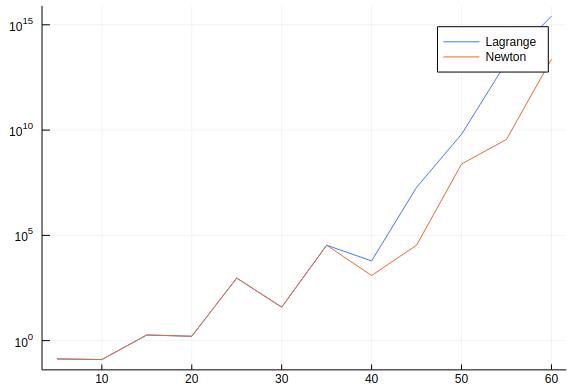
\includegraphics[width=\linewidth]{lagnew.png}
  \caption{Porównanie dokładności postaci Newtona i Lagrange'a dla funkcji Rungego}
  \label{lagnew}
\end{figure} 

Poniżej przedstawiono pomiary dla funkcji Rungego. Pomiary przebiegają
co 5 stopni wielomianu interpolacyjnego, na przedziale $(-1,1)$ liczony jest błąd
jako różnica w pomiędzy wielomianem interpolującym postaci a funkcją.
Przedstawione jest to odpowiednio dla postaci Newtona i Lagrange. 
Różnica wyrażona jest jako całka oznaczona na przedziale $(-1,1)$.
Wykres \ref{lagnew} został przedstawiony w skali logarytmicznej, aby pokazać od którego miejsca
widoczna jest różnica pomiędzy postaciami.
Widać, że postać Newtona daje dokładniejsze wyniki od postaci Lagrange'a.

\subsubsection{Stosunek błędu}
Widząc, że postać Newtona jest dokładniejsza od postaci Lagrange'a można jeszcze zobaczyć jak bardzo się różnią.
Wykres \ref{stos} przedstawia stosunek błędów interpolacji postaci Lagrange'a do Newtona. Widać, że
już dla trochę większych stopni wielomianu interpolującego (między 40 a 60) postać Newtona może być kilkaset lub nawet
kilka tysięcy razy dokładniejsza od postaci Lagrange'a. Wykres został przedstawiony również w skali logarytmicznej.
\begin{figure}[h!]
  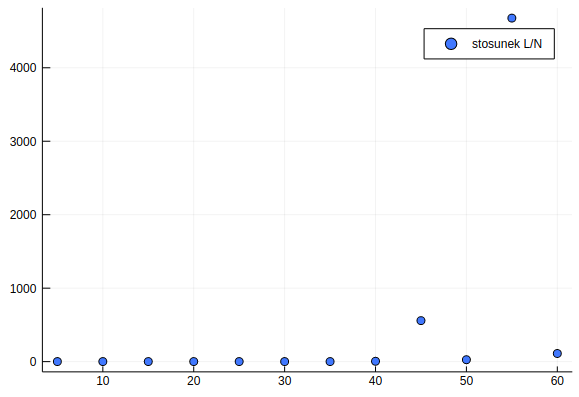
\includegraphics[width=120mm]{stosunek.png}
  \caption{Stosunek błędów postaci Lagrange'a do Newtona}
  \label{stos}
\end{figure} 
\begin{figure}[h!]
  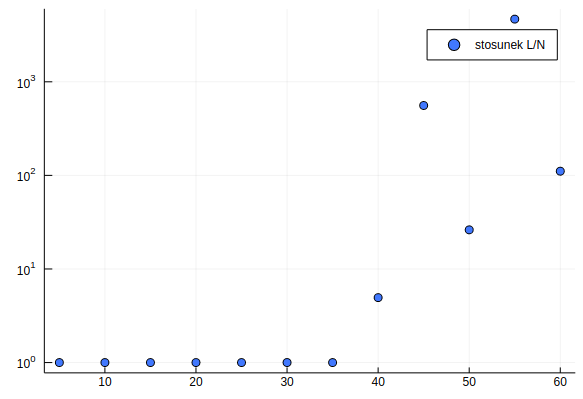
\includegraphics[width=120mm]{stosunek_log.png}
  \caption{Stosunek błędów postaci Lagrange'a do Newtona w skali logarytmicznej}
  \label{stos_log}
\end{figure} 

\subsection{Porównanie funkcji}
Błąd dokładności zależy od stopnia wielomianu interpolującego, ale także od interpolowanej funkcji.
Poniższa tabela przedstawia różnicę pomiędzy wielomianem interpolującym n-tego stopnia, a funkcjami:
$sin(x)$, $arctan(x)$, $runge(x)$.
\begin{center}
\begin{tabular}{ |c|c|c|c| } 
 \hline
 n & runge & atan & sin \\ 
 25 & 937.84 & 6.03e-5 & 5.18e-5 \\ 
 30 & 39.071 & 0.0511 & 0.0513 \\
 35 & 34061 & 55.011 & 53.414 \\
 40 & 1239.1 & 13009 & 12575 \\
 45 & 34169.05 & 150401.42 & 159703.12 \\ 
 \hline
\end{tabular}
\end{center}
Widać, że funkcje, które wydawały się zachowywać podobnie ($rg(x)$ i $arctan(x)$), przyjmują
różne wartości błędów, natomiast błędy interpolacji funkcji $sin(x)$ są bardzo bliskie błędom
$arctan(x)$. W takim razie lepiej jest badać jedną ustaloną funkcję, gdyż o wiele większy wpływ
na błąd interpolacji ma stopień interpolującego wielomianu, niż funkcja, którą chcemy interpolować.

\section{Wnioski}
Dla uzyskanych pomiarów postać interpolacyjna Newtona okazała się dokładniejsza od postaci Lagrange'a.
Różnice nie są widoczne dla małych stopni interpolującego wielomianu (do ok. 30), ale potem znacznie rosną.
Chcąc interpolować funkcję wielomianem w wielu punktach lepiej jest użyć do tego postaci Newtona.


\begin{thebibliography}{9}

\bibitem{artykul}
  Wilhelm Werner
  \textit{Polynomial Interpolation: Lagrange versus Newton}, \\
  Mathematics of Computation, volume 43, number 167, July 1984
\end{thebibliography}

\end{document}
